\documentclass{standalone}
\usepackage{pgf}
\usepackage[english]{babel}
\usepackage[utf8]{inputenc}
%\usepackage{beamerthemesplit}
\usepackage{graphics,epsfig, subfigure}
\usepackage{url}
\usepackage{srcltx}
\usepackage{hyperref}
\usepackage{mathtools}
\usepackage{amsfonts}
\usepackage{amsmath}
\usepackage{physics}
\begin{document}
$
	A_6=\sum_{\text{cyclic}}~~\raisebox{-6.5mm}{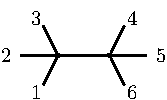
\includegraphics[trim={0cm 0cm 0cm 0cm},clip,scale=1]{fac-cycle}}~+~\raisebox{-8.9mm}{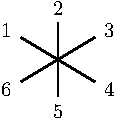
\includegraphics[trim={0cm 0cm 0cm 0cm},clip,scale=1]{contact-cycle}}
$
\end{document}